
\documentclass{article}
\newcommand{\path}{../../assets/settings}
\input{\path/newcommand.tex}
\input{\path/usepackage.tex}
\input{\path/quitarnumerossecciones.tex}

% \usepackage{nopageno} % Paquete para desactivar la numeración de páginas

\title{Distancia mínima entre filas de módulos}
\author{Kgnete}
\date{\today}

\begin{document}

\maketitle
%%%%%%%%%%%%%%%%%%%%%%%%%%%%%%%%%%%%%%%%%%%%%%%%%%%%%%%%%%%%%%%%%%%%%%%%%%%%%%%

\subsection{Distancia mínima entre filas de módulos    }
\footnote{    IDAE. 
Instalaciones de
Energía Solar Fotovoltaica.
Pliego de Condiciones Técnicas de
Instalaciones Conectadas a Red
PCT-C-REV - julio 2011}


La distancia d, medida sobre la horizontal, entre filas de módulos o entre una fila y un obstáculo
de altura h que pueda proyectar sombras, se recomienda que sea tal que se garanticen al menos
4 horas de sol en torno al mediodía del solsticio de invierno.
En cualquier caso, d ha de ser como mínimo igual a $h \cdot k$,, siendo k un factor adimensional al que,
en este caso, se le asigna el valor $1/\tan(61°- latitud)$.
En la tabla pueden verse algunos valores significativos del factor k, en función de la latitud
del lugar.
%%%%%%%%%%%%%%%%%%%%%%%%%%%%%%%%%%%%%%%%%%%%%%%%%%
\begin{table}[H]
    \centering
    \begin{tabular}{|c|c|c|c|c|c|c|}
        \hline
        \textbf{Latitud} & \textbf{29\textdegree} & \textbf{37\textdegree} & \textbf{39\textdegree} & \textbf{41\textdegree} & \textbf{43\textdegree} & \textbf{45\textdegree} \\ \hline
        $k$ & 1,600 & 2,246 & 2,475 & 2,747 & 3,078 & 3,487 \\ \hline
    \end{tabular}
\end{table}
%%%%%%%%%%%%%%%%%%%%%%%%%%%%%%%%%%%%%%%%%%%%%%%%%%

Asimismo, la separación entre la parte posterior de una fila y el comienzo de la siguiente no será
inferior a $h \cdot k$, siendo en este caso h la diferencia de alturas entre la parte alta de una fila y la
parte baja de la posterior, efectuándose todas las medidas con relación al plano que contiene las
bases de los módulos.



%%%%%%%%%%%%%%%%%%%%%%%%%%%%%%%%%%%%%%%%%%%%%%%%%%
\begin{figure}[h]
    \centering
    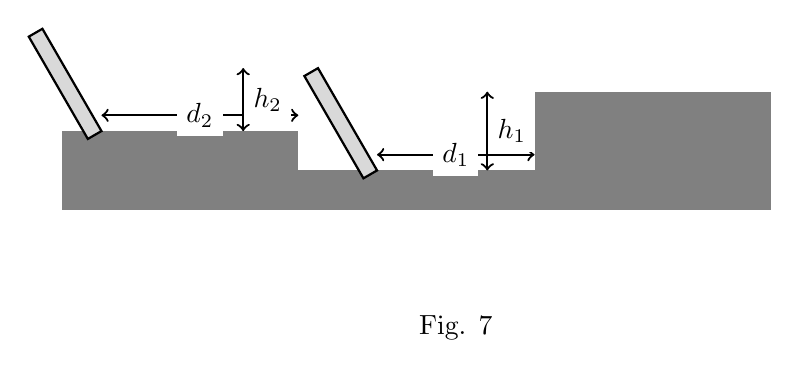
\begin{tikzpicture}
        % Definir coordenadas y ángulos
        \def\d{3} % distancia horizontal
        \def\h{2} % altura
        \def\angle{120} % ángulo de inclinación de las placas
        \def\length{1.5} % longitud de las placas

       % Dibujar el suelo y plataformas con rayado
    %    \fill[pattern=north east lines] (-2,-0.5) rectangle (10,0);
    \fill[color=gray](0,0) -- (0,1) -- (\d,1) -- (\d,0) -- cycle;
    \fill[color=gray] (\d,0) -- (\d,.5) -- (\d*2,.5) -- (\d*2,0) -- cycle;
    \fill[color=gray] (\d+\d,0) -- (\d+\d,1.5) -- (\d+\d+\d,1.5) -- (\d+\d+\d,0) -- cycle;

        % Definir la geometría de una placa fotovoltaica
        \begin{scope}[shift={(0.5,1)}, rotate=\angle]
            \draw[thick, fill=gray!30] (0,0) rectangle (\length,0.2);
        \end{scope}

        % Duplicar y rotar la geometría de la placa fotovoltaica
        \begin{scope}[shift={(\d+1,\h-1.5)}, rotate=\angle]
            \draw[thick, fill=gray!30] (0,0) rectangle (\length,0.2);
        \end{scope}

        % Dibujar líneas de medición y etiquetas
        \draw[<->, thick] (0.5,1.2) -- node[fill=white] {$d_2$} ++(\d-.5,0);
        \draw[<->, thick] (\d+1,.7) -- node[fill=white] {$d_1$} ++(\d-1,0);
        
        % \draw[dashed] (\d+\d, .5) -- (\d+\d,.5);  % Línea auxiliar para mostrar h
        \draw[<->, thick] (\d+\d-.6,1.5) -- node[fill=white, right] {$h_1$} ++(0,-1);

        \draw[<->, thick] (\d-.7,1) -- node[fill=white, right] {$h_2$} ++(0,.8);

        % Etiquetas de las figuras
        \node at (5,-1.5) {Fig. 7};
    \end{tikzpicture}
\end{figure}
%%%%%%%%%%%%%%%%%%%%%%%%%%%%%%%%%%%%%%%%%%%%%%%%%%

Si los módulos se instalan sobre cubiertas inclinadas, en el caso de que el azimut de estos, el de
la cubierta, o el de ambos, difieran del valor cero apreciablemente, el cálculo de la distancia
entre filas deberá efectuarse mediante la ayuda de un programa de sombreado para casos
generales suficientemente fiable, a fin de que se cumplan las condiciones requeridas.




\ifdefined\inputado % para que no meta la bibliografia de los parciales al inclustarlo con input en otro
\else
\bibliographystyle{plainnat}
\bibliography{\path/referencias}
\fi



\end{document}
